% Add \usepackage{graphicx} to your preamble if not already present.
% Place the table_replacement_figures directory beside your main .tex file.
% Use either the individual robustness figures OR the combined figure, not both.
% Figure numbers are assigned by LaTeX; update old table cross-references.

% Replaces Table IX.
\begin{figure*}[t]
\centering
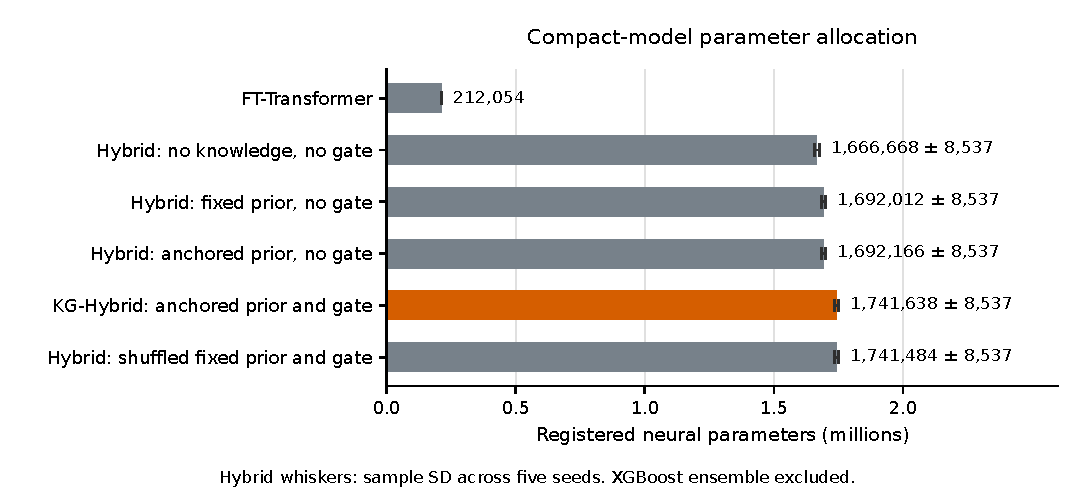
\includegraphics[width=\textwidth]{table_replacement_figures/table_ix_registered_parameters.pdf}
\caption{Registered neural parameter counts in the compact controlled comparison. Hybrid bars show means and whiskers show sample standard deviations across five seed-specific runs. The FT-Transformer count is constant across runs. Counts include the retained standalone FT classification head, which is bypassed by hybrid prediction; the separate XGBoost ensemble is excluded.}
\label{fig:registered_parameters}
\end{figure*}

% Replaces Table X.
\begin{figure}[t]
\centering
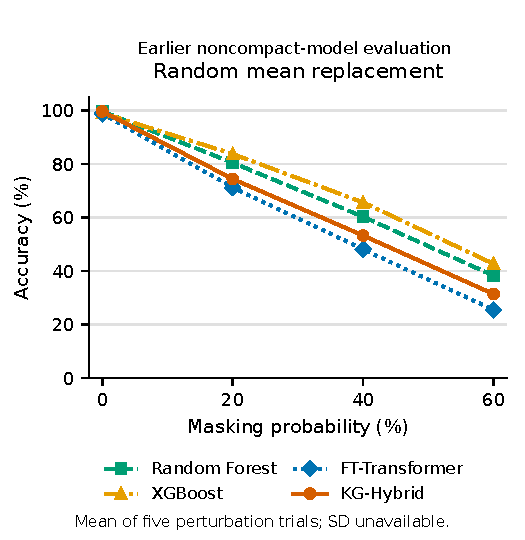
\includegraphics[width=\columnwidth]{table_replacement_figures/table_x_feature_masking.pdf}
\caption{Earlier cross-model zero-replacement experiment. Each standardized feature entry is independently replaced by zero at the indicated masking probability. Points are mean accuracies over five perturbation trials; trial-level standard deviations are unavailable. These are not results for the compact five-seed models.}
\label{fig:masking_replacement}
\end{figure}

% Replaces Table XI.
\begin{figure}[t]
\centering
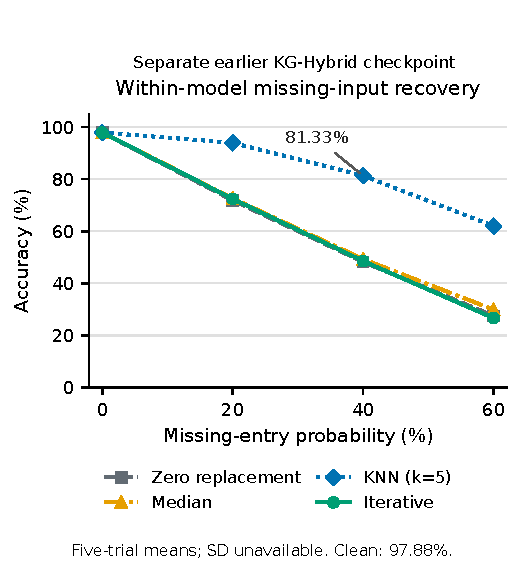
\includegraphics[width=\columnwidth]{table_replacement_figures/table_xi_imputation.pdf}
\caption{Earlier within-model KG-Hybrid imputation comparison using a separate checkpoint with clean accuracy 97.88\%. Missing entries are represented as NaNs for recovery, and all methods share the same mask within each trial. Imputers are fitted on standardized training data. Points are means over five trials; trial-level standard deviations are unavailable. This comparison does not establish an architectural advantage over imputed baselines.}
\label{fig:imputation_recovery}
\end{figure}

% Replaces Table XII.
\begin{figure}[t]
\centering
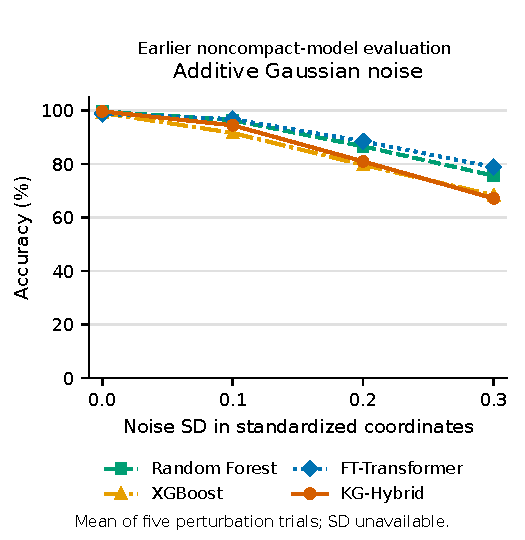
\includegraphics[width=\columnwidth]{table_replacement_figures/table_xii_gaussian_noise.pdf}
\caption{Earlier cross-model Gaussian-perturbation experiment. Independent additive noise is applied in standardized feature coordinates. Points show mean accuracies over five trials; trial-level standard deviations are unavailable. These are not compact-model results or sensor-calibrated physical noise levels.}
\label{fig:gaussian_perturbations}
\end{figure}

% Replaces Table XIII.
\begin{figure}[t]
\centering
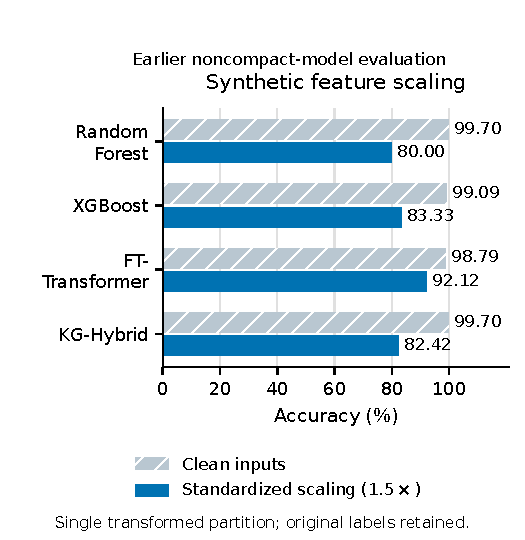
\includegraphics[width=\columnwidth]{table_replacement_figures/table_xiii_feature_scaling.pdf}
\caption{Earlier synthetic feature-scaling experiment comparing clean inputs with standardized test vectors multiplied by $1.5\times$. Values are accuracies on one deterministic evaluation partition with the original labels retained. This transformation is not external-dataset validation and does not guarantee out-of-range measurements.}
\label{fig:feature_scaling}
\end{figure}

% Replaces Tables X, XII and XIII.
\begin{figure*}[t]
\centering
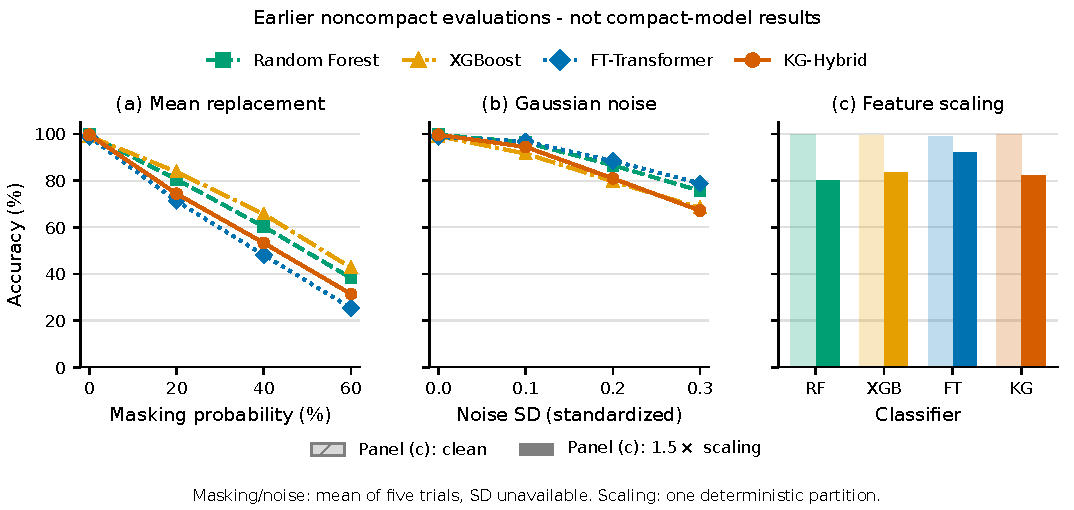
\includegraphics[width=\textwidth]{table_replacement_figures/combined_robustness_three_panel.pdf}
\caption{Earlier noncompact-model stress tests: (a) independent zero replacement of standardized feature entries, (b) independent additive Gaussian noise in standardized coordinates, and (c) clean inputs versus $1.5\times$ standardized feature scaling. Panels (a) and (b) show means over five perturbation trials, without available trial-level standard deviations; panel (c) uses one deterministic transformed partition. Original benchmark labels are retained. These results do not describe the compact five-seed models. The separate within-model imputation comparison is not included.}
\label{fig:combined_robustness}
\end{figure*}
